The \acrfull{iot} is an umbrella term used to describe physical `smart' devices
equipped with telecommunication interfaces, connected to one another via the 
Internet \citep{centenaro_long-range_2016}.
Whereas the Internet traditionally connected computers, the embedding of 
electronics into physical objects has allowed the Internet to expand \citep{miorandi_internet_2012}.
These devices can contain sensors which will produce data and in some cases 
these devices can be controlled remotely. The combination of these devices in
a network, especially when the actions of one devices are informed by the 
data from another device, is the foundation of \gls{iot} \citep{minerva_towards_2015}.
\gls{iot} systems can impact in many areas such as home automation,
where devices can work together to automate heating and security aspects of 
the home \citep{lee_internet_2018}, and medicine where devices
can be used as monitors to provide real time information about 
patient health \citep{kumar_iot_2016}.

\begin{figure}[H]
    \centering
    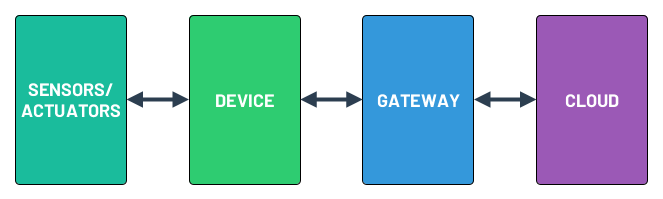
\includegraphics[width=\imageWidth\textwidth]{assets/generic_iot_architecture.png}
    \caption{\label{fig:generic_iot_architecture} Basic \gls{iot} Architecture.}
\end{figure}

\figref{fig:generic_iot_architecture} illustrates the various components present
within any given \gls{iot} architecture. The sensor/actuator is the component
that will receive data from the real world or perform a physical action. This 
data is then transmitted to a device which is responsible for the sensor/actuator.
This device may be responsible for multiple sensors, as in \citet{jassas_smart_2015}
which connected multiple e-health sensors to a \gls{rpi} device. This device will
then communicate with a gateway. The gateway will handle the destination of data passed
to it. Within \gls{coap} the gateway would be a router ensuring messages are sent 
to the correct endpoints. The cloud is final destination for the sensor data where
the data will be stored and can be further used for analysis.
